
\begin{figure}[H]
	\centering
	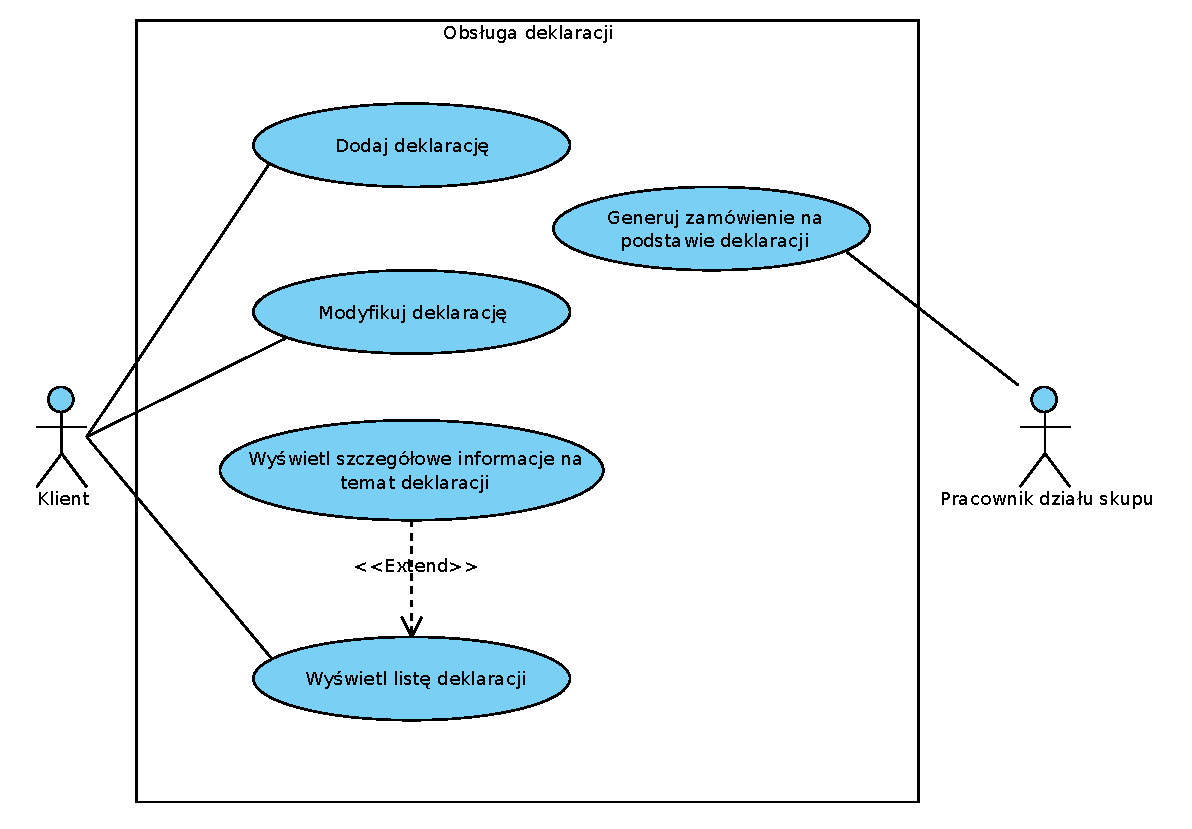
\includegraphics[width=1.1\textwidth]{img/UC/deklaracje.eps}
\end{figure}

\begin{usecase}{Dodaj deklarację}
	\textbf{Autor:} Klient \\
	\textbf{Cel przypadku użycia:} dodanie deklaracji w celu jej realizacji \\
	\textbf{Kontekst użycia:} chęć dodania deklaracji \\
	\textbf{Zakres:} System obsługi klienta \\
	\textbf{Poziom:} biznesowy \\
	\textbf{Aktor główny:} Klient \\
	\textbf{Wyzwalacz:} wybranie zakładki dodawania deklaracji \\
	\textbf{Warunek początkowy:} klient jest zalogowany i ma uprawnienia do dodawania deklaracji \\
	\textbf{Minimalna gwarancja:} w przypadku nieprzyjęcia deklaracji klient zostanie poinformowany o problemie \\
	\textbf{Główny scenariusz powodzenia:} \\
		\begin{enumerate}
			\item Klient wprowadza rok, na który chce deklarować
			\item Klient poprawnie wybiera miesiące, na które chce deklarować
			\item Klient wybiera kategorię odpadów z listy kategorii
			\item System wyświetla listę odpadów z danej kategorii, które zostały zawarte w umowie z klientem
			\item Klient wybiera odpady, które chce zadeklarować
			\item Klient poprawnie wprowadza ilości i/lub wagi wybranych odpadów
			\item Klient wybiera opcję wysłania deklaracji
			\item System pozytywnie weryfikuje poprawność deklaracji
			\item System zapisuje deklarację w systemie
			\item System wyświetla informację o poprawnym zapisaniu deklaracji w systemie
		\end{enumerate}
	\textbf{Rozszerzenia:} \\
		2.1. Klient wybrał miesiące, na które istnieją już deklaracje \\
			\indent 2.1.1. System wyświetla informację o niemożliwości dodanie deklaracji \\
		4.1. Klient wybiera opcję wyświetlania wszystkich odpadów \\
			\indent 4.1.1. System wyświetla listę wszystkich odpadów z danej kategorii \\
			\indent 4.1.2. Klient wybiera odpady, które chce zadeklarować \\
			\indent 4.1.3. System wysyła informację do opiekuna klienta o potrzebie podpisania aneksu do umowy -> pt 6 \\
		6.1. Klient wprowadza błędną ilość odpadów -> System wyświetla informację o błędnych danych \\
		8.1. System negatywnie weryfikuje poprawność deklaracji -> Wyświetla informację o błędnych danych \\
		10.1. System wyświetla informację o błędzie zapisu do bazy danych \\
\end{usecase}

\begin{usecase}{Modyfikuj deklarację}
	\textbf{Autor:} Klient\\
	\textbf{Cel przypadku użycia:} Modyfikacja dodanego przez tego klienta deklaracji \\
	\textbf{Kontekst użycia:} chęć modyfikacji istniejącej deklaracji\\
	\textbf{Zakres:} System obsługi klienta \\
	\textbf{Poziom:} biznesowy \\
	\textbf{Aktor główny:} Klient\\
	\textbf{Wyzwalacz:} naciśnięcie odpowiedniego przycisku na stronie www \\
	\textbf{Warunek początkowy:} klient jest zalogowany\\
	\textbf{Minimalna gwarancja:} w przypadku, gdy deklaracja nie zostanie zmodyfikowana, klient dostanie odpowiedni komunikat \\
	\textbf{Główny scenariusz powodzenia:} \\
		\begin{enumerate}
			\item Klient klika w przycisk "modyfikuj"
			\item Po dokonaniu zmian, klika "wyślij"
			\item Dostaje komunikat o powodzeniu akcji
		\end{enumerate}
			3.1 Dostaje odpowiedni komunikat o niepowodzeniu
\end{usecase}

\begin{usecase}{yświetl listę deklaracji}
	\textbf{Autor:} Klient\\
	\textbf{Cel przypadku użycia:} Wylistowanie deklaracji złożonych przez klienta \\
	\textbf{Kontekst użycia:} chęć przejżenia deklaracji\\
	\textbf{Zakres:} System obsługi klienta \\
	\textbf{Poziom:} biznesowy \\
	\textbf{Aktor główny:} Klient\\
	\textbf{Wyzwalacz:} naciśnięcie odpowiedniego przycisku na stronie www \\
	\textbf{Warunek początkowy:} klient jest zalogowany\\
	\textbf{Minimalna gwarancja:} wyświetlenie ostatnich deklaracji\\
	\textbf{Główny scenariusz powodzenia:} \\
		\begin{enumerate}
			\item Klient klika w przycisk "lista deklaracji"
			\item Klient dostaje listę
		\end{enumerate}
\end{usecase}

\begin{usecase}{Wyświetl szczegółowe informacje na temat deklaracji}
	\textbf{Autor:} Klient\\
	\textbf{Cel przypadku użycia:} Wyświetlenie szczegółów wybranej deklaracji \\
	\textbf{Kontekst użycia:} chęć dostania szczegółowych informacji o deklaracji\\
	\textbf{Zakres:} System obsługi klienta \\
	\textbf{Poziom:} biznesowy \\
	\textbf{Aktor główny:} Klient\\
	\textbf{Wyzwalacz:} naciśnięcie odpowiedniego przycisku na stronie www \\
	\textbf{Warunek początkowy:} klient jest zalogowany i ma wyświetloną listę deklaracji\\
	\textbf{Minimalna gwarancja:} wyświetlenie szczegółów deklaracji \\
	\textbf{Główny scenariusz powodzenia:} \\
		\begin{enumerate}
			\item Klient klika w przycisk "szczegóły"
			\item Dostaje szczegółowe informacje
		\end{enumerate}
\end{usecase}

\begin{usecase}{Generuj zamówienie na podstawie deklaracji}
	\textbf{Autor:} Pracownik działu skupu\\
	\textbf{Cel przypadku użycia:} Wygenerowanie zamówienia \\
	\textbf{Kontekst użycia:} chęć wygenerowania zamówienia na podstawie danej deklaracji\\
	\textbf{Zakres:} System obsługi klienta \\
	\textbf{Poziom:} biznesowy \\
	\textbf{Aktor główny:} Pracownik działu skupu\\
	\textbf{Wyzwalacz:} wybór deklaracji i kliknięcia opcji generuj \\
	\textbf{Warunek początkowy:} wybrana deklaracja \\
	\textbf{Minimalna gwarancja:} w przypadku, gdy zamówienie nie zostanie wygenerowane, Pracownik dostanie odpowiedni komunikat \\
	\textbf{Główny scenariusz powodzenia:} \\
		\begin{enumerate}
			\item Pracownik klika w przycisk "generuj"
			\item Dostaje komunikat o powodzeniu akcji
		\end{enumerate}
	\textbf{Rozszerzenia:} \\
			2.1 Dostaje odpowiedni komunikat o niepowodzeniu
\end{usecase}

\begin{figure}[H]
	\centering
	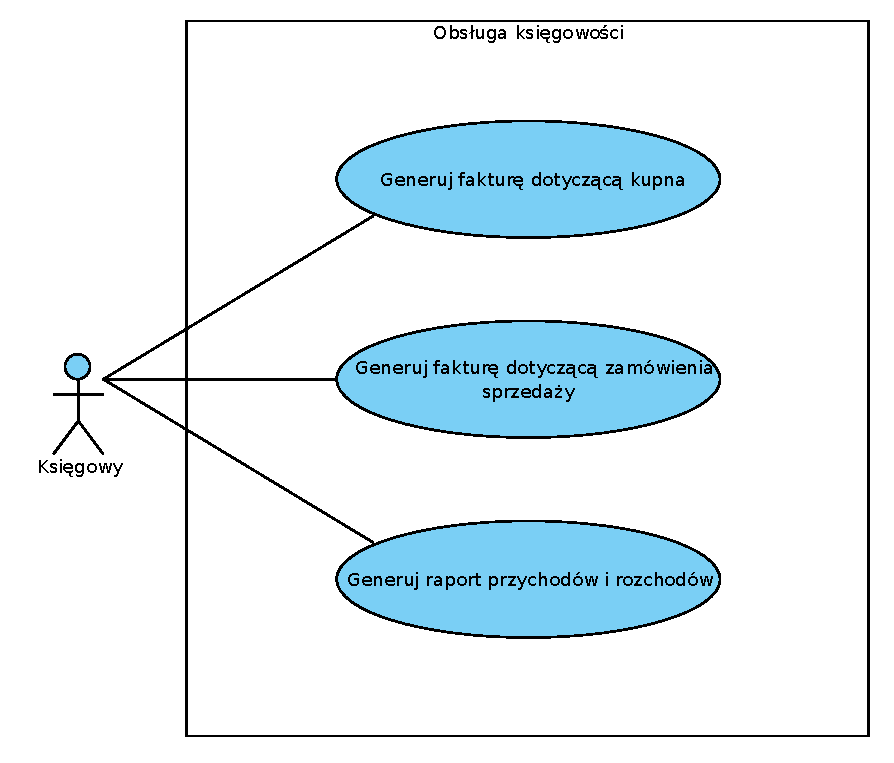
\includegraphics[width=.8\textwidth]{img/UC/ksiegowosc.eps}
\end{figure}

<<<<<<< HEAD
\textbf{Numer i Nazwa przypadku użycia:} UC05 - Generuj fakturę sprzedaży produktów recyklingu \\
\textbf{Autor:} Księgowy\\
\textbf{Cel przypadku użycia:} Wygnerowanie faktury \\
\textbf{Kontekst użycia:} otrzymanie dokumentu dowodu sprzedaży produktów  \\
\textbf{Zakres:} system księgujący \\
\textbf{Poziom:} biznesowy \\
\textbf{Aktor główny:} Księgowy \\
\textbf{Wyzwalacz:} sprzedaż produktów recyklingu \\
\textbf{Warunek początkowy:} księgowy posiada identyfikator zamówienia \\
\textbf{Minimalna gwarancja:} w przypadku, gdy nie będzie można wygenerować faktury, system poinformuje o tym aktora, nie generując błędnego dokumentu \\
\textbf{Główny scenariusz powodzenia:} 
	\begin{enumerate}
		\item Księgowy wpisuje identyfikator zamówienia
		\item System sprawdza czy w systemie jest zamówienie, o danym identyfikatorze
		\item System generuje fakturę 
	\end{enumerate}
\textbf{Rozszerzenia:} \\
2.1 Jeżeli identyfikator jest niepoprawny, system informuje o tym księgowego i prosi go o ponowne podanie tego parametru

\textbf{Numer i Nazwa przypadku użycia:} UC06 - Generuj fakturę dotyczącą usłiugi przejęcia obowiązku recyklingu \\
\textbf{Autor:} Księgowy\\
\textbf{Cel przypadku użycia:} Wygnerowanie faktury \\
\textbf{Kontekst użycia:} otrzymanie dokumentu dowodu zakupu oświadczenia  \\
\textbf{Zakres:} system księgujący \\
\textbf{Poziom:} biznesowy \\
\textbf{Aktor główny:} Księgowy \\
\textbf{Wyzwalacz:} kupno oświadczenia oddzysku \\
\textbf{Warunek początkowy:} księgowy posiada identyfikator danych dotyczących odpowiedniej oferty sprzedaży \\
\textbf{Minimalna gwarancja:} w przypadku, gdy nie będzie można wygenerować faktury, system poinformuje o tym aktora, nie generując błędnego dokumentu \\
\textbf{Główny scenariusz powodzenia:} 
	\begin{enumerate}
		\item Księgowy wpisuje identyfikator do oferty sprzedaży
		\item System sprawdza czy w systemie jest oferta, o danym identyfikatorze
		\item System generuje fakturę 
	\end{enumerate}
\textbf{Rozszerzenia:} \\
2.1 Jeżeli identyfikator jest niepoprawny, system informuje o tym księgowego i prosi go o ponowne podanie tego parametru

\textbf{Numer i Nazwa przypadku użycia:} UC07 - Wprowadź dane faktury kupna oświadzczenia o przetworzeniu odpadów \\
\textbf{Autor:} Księgowy\\
\textbf{Cel przypadku użycia:} Wpisanie do systemu danych o fakturze \\
\textbf{Kontekst użycia:} posiadanie w bazie wszystkich informacji o operacjach firmy\\
\textbf{Zakres:} system księgujący \\
\textbf{Poziom:} biznesowy \\
\textbf{Aktor główny:} Księgowy \\
\textbf{Wyzwalacz:} kupno oświadczenia oddzysku \\
\textbf{Warunek początkowy:} księgowy posiada dane o fakturze kupna oświadczenia o przetworzeniu odpadów \\
\textbf{Minimalna gwarancja:} w przypadku, gdy nie będzie można wproawdzić danych do bazy, nie zostanie ona zmodyfikowana \\
\textbf{Główny scenariusz powodzenia:} 
	\begin{enumerate}
		\item Księgowy wpisuje dane z faktury do systemu
		\item System sprawdza czy format poszczególnych danych jest prawidłowy
		\item System wprowadza dane do systemu
	\end{enumerate}
\textbf{Rozszerzenia:} \\
2.1 Jeżeli jakieś dane są niepoprawne, księgowy zostaje o tym poinformowany i musi wprowadzić je ponownie

\textbf{Numer i Nazwa przypadku użycia:} UC08 - Generuj raport przychodów i rozchodów \\
\textbf{Autor:} Księgowy\\
\textbf{Cel przypadku użycia:} Wygnerowanie raportu o zyskach i stratach firmy \\
\textbf{Kontekst użycia:} otrzymanie raportu dla właściciela  \\
\textbf{Zakres:} system księgujący \\
\textbf{Poziom:} biznesowy \\
\textbf{Aktor główny:} Właściciel \\
\textbf{Aktor uczestniczący:} Księgowy \\
\textbf{Wyzwalacz:} właściciel chce mieć informację o przychodach i rozchodach firmy w danym okresie czasowym \\
\textbf{Warunek początkowy:} podanie ram czasowych  \\
\textbf{Minimalna gwarancja:} w przypadku, gdy nie będzie można wygenerować raportu, system poinformuje o tym właściciela, nie generując błędnych informacji \\
\textbf{Główny scenariusz powodzenia:} 
	\begin{enumerate}
		\item Właściciel podaje ramy czasowe okresu, ktory go interesuje
		\item System wybiera tylko te faktury, które zawierają się w podanym przedziale czasowym
		\item System generuje raport
	\end{enumerate}
\textbf{Rozszerzenia:} \\
1.1 Ramy czasowe są błędne - conajmniej jedna z wartości jest w przyszłości, system wygeneruje błąd i poprosi o ich ponowne wpisanie

\begin{usecase}{Generuj fakturę sprzedaży produktów recyklingu}
	\textbf{Autor:} Księgowy\\
	\textbf{Cel przypadku użycia:} Wygnerowanie faktury \\
	\textbf{Kontekst użycia:} otrzymanie dokumentu dowodu sprzedaży produktów  \\
	\textbf{Zakres:} system księgujący \\
	\textbf{Poziom:} biznesowy \\
	\textbf{Aktor główny:} Księgowy \\
	\textbf{Wyzwalacz:} sprzedaż produktów recyklingu \\
	\textbf{Warunek początkowy:} księgowy posiada identyfikator zamówienia \\
	\textbf{Minimalna gwarancja:} w przypadku, gdy nie będzie można wygenerować faktury, system poinformuje o tym aktora, nie generując błędnego dokumentu \\
	\textbf{Główny scenariusz powodzenia:} 
		\begin{enumerate}
			\item Księgowy wpisuje identyfikator zamówienia
			\item System sprawdza czy w systemie jest zamówienie, o danym identyfikatorze
			\item System generuje fakturę 
		\end{enumerate}
	\textbf{Rozszerzenia:} \\
	2.1 Jeżeli identyfikator jest niepoprawny, system informuje o tym księgowego i prosi go o ponowne podanie tego parametru
\end{usecase}

\begin{usecase}{Generuj fakturę dotyczącą usłiugi przejęcia obowiązku recyklingu}
	\textbf{Autor:} Księgowy\\
	\textbf{Cel przypadku użycia:} Wygnerowanie faktury \\
	\textbf{Kontekst użycia:} otrzymanie dokumentu dowodu zakupu oświadczenia  \\
	\textbf{Zakres:} system księgujący \\
	\textbf{Poziom:} biznesowy \\
	\textbf{Aktor główny:} Księgowy \\
	\textbf{Wyzwalacz:} kupno oświadczenia oddzysku \\
	\textbf{Warunek początkowy:} księgowy posiada identyfikator danych dotyczących odpowiedniej oferty sprzedaży \\
	\textbf{Minimalna gwarancja:} w przypadku, gdy nie będzie można wygenerować faktury, system poinformuje o tym aktora, nie generując błędnego dokumentu \\
	\textbf{Główny scenariusz powodzenia:} 
		\begin{enumerate}
			\item Księgowy wpisuje identyfikator do oferty sprzedaży
			\item System sprawdza czy w systemie jest oferta, o danym identyfikatorze
			\item System generuje fakturę 
		\end{enumerate}
	\textbf{Rozszerzenia:} \\
	2.1 Jeżeli identyfikator jest niepoprawny, system informuje o tym księgowego i prosi go o ponowne podanie tego parametru
\end{usecase}
>>>>>>> 16f3d6beadc2a4ba4bd347295c604e10693154a3

\begin{usecase}{Wprowadź dane faktury kupna oświadzczenia o przetworzeniu odpadów}
	\textbf{Autor:} Księgowy\\
	\textbf{Cel przypadku użycia:} Wpisanie do systemu danych o fakturze \\
	\textbf{Kontekst użycia:} posiadanie w bazie wszystkich informacji o operacjach firmy\\
	\textbf{Zakres:} system księgujący \\
	\textbf{Poziom:} biznesowy \\
	\textbf{Aktor główny:} Księgowy \\
	\textbf{Wyzwalacz:} kupno oświadczenia oddzysku \\
	\textbf{Warunek początkowy:} księgowy posiada dane o fakturze kupna oświadczenia o przetworzeniu odpadów \\
	\textbf{Minimalna gwarancja:} w przypadku, gdy nie będzie można wproawdzić danych do bazy, nie zostanie ona zmodyfikowana \\
	\textbf{Główny scenariusz powodzenia:} 
		\begin{enumerate}
			\item Księgowy wpisuje dane z faktury do systemu
			\item System sprawdza czy format poszczególnych danych jest prawidłowy
			\item System wprowadza dane do systemu
		\end{enumerate}
	\textbf{Rozszerzenia:} \\
	2.1 Jeżeli jakieś dane są niepoprawne, księgowy zostaje o tym poinformowany i musi wprowadzić je ponownie
\end{usecase}

\begin{usecase}{Generuj raport przychodów i rozchodów}
	\textbf{Autor:} Księgowy\\
	\textbf{Cel przypadku użycia:} Wygnerowanie raportu o zyskach i stratach firmy \\
	\textbf{Kontekst użycia:} otrzymanie raportu dla właściciela  \\
	\textbf{Zakres:} system księgujący \\
	\textbf{Poziom:} biznesowy \\
	\textbf{Aktor główny:} Właściciel \\
	\textbf{Aktor uczestniczący:} Księgowy \\
	\textbf{Wyzwalacz:} właściciel chce mieć informację o przychodach i rozchodach firmy w danym okresie czasowym \\
	\textbf{Warunek początkowy:} podanie ram czasowych  \\
	\textbf{Minimalna gwarancja:} w przypadku, gdy nie będzie można wygenerować raportu, system poinformuje o tym właściciela, nie generując błędnych informacji \\
	\textbf{Główny scenariusz powodzenia:} 
		\begin{enumerate}
			\item Właściciel podaje ramy czasowe okresu, ktory go interesuje
			\item System wybiera tylko te faktury, które zawierają się w podanym przedziale czasowym
			\item System generuje raport
		\end{enumerate}
	\textbf{Rozszerzenia:} \\
	1.1 Ramy czasowe są błędne - conajmniej jedna z wartości jest w przyszłości, system wygeneruje błąd i poprosi o ich ponowne wpisanie
\end{usecase}

\begin{figure}[H]
	\centering
	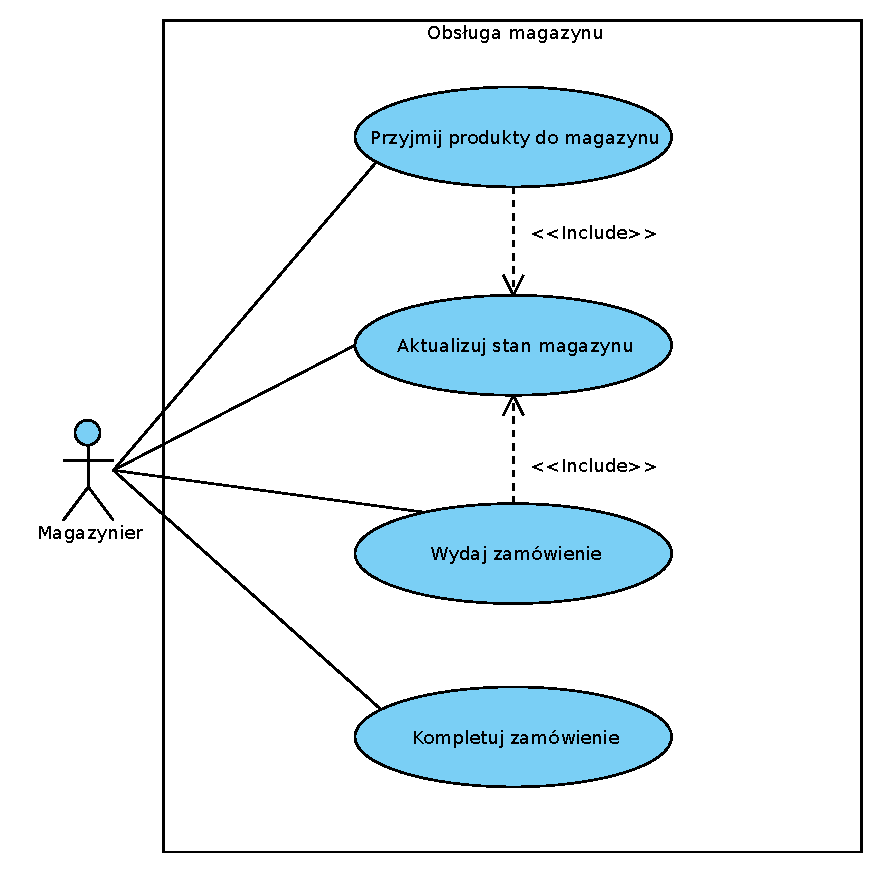
\includegraphics[width=.8\textwidth]{img/UC/magazyn.eps}
\end{figure}

\begin{usecase}{Przyjmij produkty do magazynu}
	\textbf{Autor:} Magazynier\\
	\textbf{Cel przypadku użycia:} Dodanie produktów recyklingu do magazynu i aktualizacja stanu magazynu \\
	\textbf{Kontekst użycia:} przechowanie produktów recyklingu w magazynie\\
	\textbf{Zakres:} system magazynowy \\
	\textbf{Poziom:} biznesowy \\
	\textbf{Aktor główny:} Magazynier \\
	\textbf{Uczestnicy:} Kierowca \\
	\textbf{Wyzwalacz:} dostarczenie przez kierowce produktów do magazynu \\
	\textbf{Warunek początkowy:} kierowca ma produkty recyklingu, które należy zmagazynować oraz ich listę \\
	\textbf{Minimalna gwarancja:} w przypadku, gdy produkty nie zostaną zmagazynowane, stan magazynu nie będzie zmieniany \\
	\textbf{Główny scenariusz powodzenia:} \\
		\begin{enumerate}
			\item Kierowca przywozi produkty
			\item Magazynier układa je w magazynie
			\item Magazynier aktualizuje stan magazynu
		\end{enumerate}
\end{usecase}

\begin{usecase}{Wydaj zamówienie}
	\textbf{Autor:} Magazynier\\
	\textbf{Cel przypadku użycia:} Wydanie kierowcy produktów, ujętych w zamówieniu \\
	\textbf{Kontekst użycia:} potrzeba przetransporotowania produktów do kupca\\
	\textbf{Zakres:} system magazynowy \\
	\textbf{Poziom:} biznesowy \\
	\textbf{Aktor główny:} Magazynier \\
	\textbf{Uczestnicy:} Kierowca \\
	\textbf{Wyzwalacz:} przyjazd kierowcy do magazynu \\
	\textbf{Warunek początkowy:} kierowca ma zamówienie \\
	\textbf{Minimalna gwarancja:} w przypadku, gdy nie można skompletować zamówienia stan magazynu się nie zmieni \\
	\textbf{Główny scenariusz powodzenia:} 
		\begin{enumerate}
			\item Kierowca przekazuje numer zamówienia magazynierowi
			\item Magazynier wydaje produkty kierowcy
			\item Magazynier uaktualnia stan magazynu
		\end{enumerate}
	\textbf{Rozszerzenia:} \\
	1.1 W przypadku gdy magazynier nie otrzymał wcześniej informacji o zamówieniu, kompletuje je teraz, w razie niepowodzenia produkty nie zostają wydane\\
\end{usecase}

\begin{usecase}{Aktualizuj stan magazynu}
	\textbf{Autor:} Magazynier\\
	\textbf{Cel przypadku użycia:} Aktualizacja danych o stanie magayznu \\
	\textbf{Kontekst użycia:} utrzymywanie aktualnej informacji o ilości produktów w magazynie \\
	\textbf{Zakres:} system magazynowy \\
	\textbf{Poziom:} użytkowy \\
	\textbf{Aktor główny:} Magazynier \\
	\textbf{Wyzwalacz:} wydanie lub przyjęcie produktów \\
	\textbf{Warunek początkowy:} zmiana stanu magazynu \\
	\textbf{Minimalna gwarancja:} w przypadku, gdy nie można zaktualizować stanu magazynu, jego stan pozostanie niezmieniony \\
	\textbf{Główny scenariusz powodzenia:} 
		\begin{enumerate}
			\item Magazynier wpisuje informację o wydanych/przyjętych produktach
		\end{enumerate}
\end{usecase}

\begin{usecase}{Kompletuj zamówienie}
	\textbf{Autor:} Magazynier\\
	\textbf{Cel przypadku użycia:} Skompletowanie zamówienie w celu wydania go kierowcy \\
	\textbf{Kontekst użycia:} chęć uporządkowania produktów do zamówienia w celu szybkiego ich przekazania kierowcy \\
	\textbf{Zakres:} system magazynowy \\
	\textbf{Poziom:} biznesowy \\
	\textbf{Aktor główny:} Magazynier \\
	\textbf{Wyzwalacz:} dostanie informacji o zamówieniu \\
	\textbf{Warunek początkowy:} odpowiednia ilość towarów w magazynie \\
	\textbf{Minimalna gwarancja:} w przypadku, gdy nie ma odpowiedniej ilości towarów w magazynie, zostanie wysłana informacja zwrotna  \\
	\textbf{Główny scenariusz powodzenia:} 
		\begin{enumerate}
			\item Magazynier otrzymuje listę towarów, które wchodzą w skład zamówienia
			\item Magazynier sprawdza czy posiada ich odpowiednią ilość
			\item Magazynier przygotowuje zamówienie
		\end{enumerate}
	\textbf{Rozszerzenia:} \\
	2.1. Nie można skompletować zamówienia, zostaje wysłana informacja zwrotna o nieposiadanych towarach\\
\end{usecase}

